\documentclass[11pt,a4paper]{article}
\usepackage{booktabs}
\usepackage{caption}  
\usepackage{changepage}
\usepackage{geometry}
 \usepackage{pgfplots}
 \usepgfplotslibrary{dateplot}
\usepackage{diagbox}
\usepackage{tcolorbox}
\usepackage{xpinyin}
\usepackage{subfigure}
\usepackage{float}
\usepackage{multicol}
\usepackage{multirow}
\usepackage[T1]{fontenc}
\usepackage[utf8]{inputenc}
\usepackage{authblk}
\usepackage{threeparttable}
\usepackage{amsmath}

\geometry{top=2cm,bottom=2cm,left=2cm,right=2cm}

\title{Math 286 Lab Project}
\date{2020, Sept, 11th}
\author{\textbf{Ruan Yucheng} 3180111}
\author{\textbf{Zhang Zheyuan} 3180111607}
\author{\textbf{Wu Zheyu} 3180111}
\author{\textbf{Qian Chen} 3180111591}
\author{\textbf{Zheng Xiuwen} 3180111}
\affil{Department of Mechanical Engineering, ZJUI}
\renewcommand\Authands{ and }

\begin{document}
\maketitle

\section{Problem 1}
Determine the maximal solution of the following ODE with the initial value.
\begin{equation}
	y' = t^2+y^3, y(0)=1	\tag{IVP1}  \label{IVP1}
\end{equation}
\subsection{Direction Field}
At first, we plot the direction field of (1). After connecting the direction arrows we find that the curve seems has 2 vertical asymptotes, which approximately lies between -2.1 to -2.2 and 0.8 to 0.9.

\begin{center}
	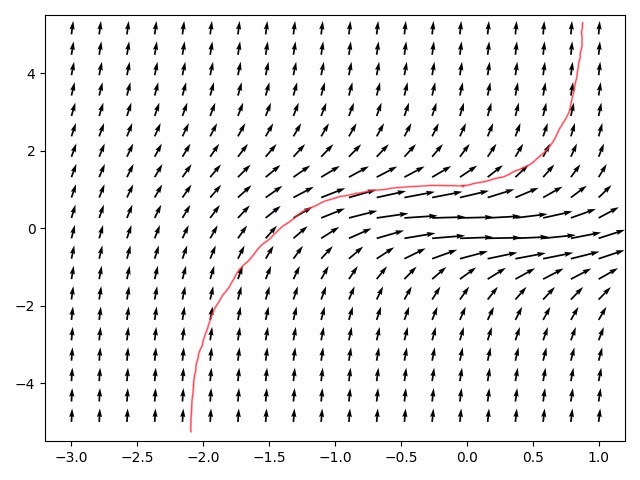
\includegraphics[scale=0.3]{HandSketch.jpeg}
\end{center}

\subsection{Numerical Methods}

\subsubsection{Methods}
\begin{table}[!htb]
	\begin{center}
		\scriptsize
		\renewcommand{\arraystretch}{1.3} % default is 1.0
		\begin{tabular}{p{8cm}|p{8cm}}
			\textbf{Euler}: <code>			& \quad\textbf{Heun}: <code>				\\
			$y_{n+1} = y_n+h*f(t_n, y_n)$	& \quad$ k_{1,n} = f(t_n,y_n)$				\\
			$ t_{n+1} = t_n+h$				& \quad$ k_{2,n} = f(t_n+h, y_n+h*k_{1,n})$	\\
											& \quad$ y_{n+1} = y_n+h*f(t_n, y_n)$		\\
											& \quad$ t_{n+1} = t_n+h$					\\
										 	
			
			\textbf{Runge Kutta}: <code>										&					\\
			$ k_{1,n} = f(t_n,y_n)$												&					\\
			$ k_{2,n} = f(t_n+\frac{h}{2}, y_n+\frac{h}{2}*k_{1,n})$			&					\\
			$ k_{3,n} = f(t_n+\frac{h}{2}, y_n+\frac{h}{2}*k_{2,n})$			&					\\
			$ k_{4,n} = f(t_n+h, y_n+h*k_{3,n})$								&					\\
			$ y_{n+1} = y_n+\frac{h}{6}*(k_{1,n}+2*(k_{2,n}+k_{3,n})+k_{4,n})$	&					\\
			$ t_{n+1} = t_n+h$													&					\\
			
		\end{tabular}
	\end{center}
\end{table}

\subsubsection{Approximation}
\noindent We apply three methods all together with a step of $h = 0.1$ obtain the table below:
\begin{table}[!htb]
	\begin{center}
		\scriptsize
		\renewcommand{\arraystretch}{1.5} % default is 1.0
		\begin{tabular}{l|r|r|r|r|r|r|r|r}
			\textbf{T}	&\textbf{-2.3}	&\textbf{-2.2}	&\textbf{-2.1}	&\textbf{-2.0}	&\textbf{0.7}	&\textbf{0.8}	&\textbf{0.9}	&\textbf{1.0}	\\
			\hline
			Euler		&-19.87			&-9.10			&-5.05			&-3.08			&3.41			&4.85			&7.66			&14.31			\\	
			\hline
			Heun		&-5.48E5		&-175.74		&-17.44			&-6.25			&5.36			&11.14			&48.95			&4479.18		\\
			\hline
			RK			&-1.62E99		&-2.59E7		&-36.57			&-7.12			&5.89			&16.04			&2777.84		&5.43E35		\\
		\end{tabular}
	\end{center}
\end{table}

Combined with the table, the direction field and the hand-drawing sketches, we could find that the results diverses dramatically large around -2.2 to -2.1 and 0.8 to 0.9. Which may conform with our initial observation. To verify this we apply three methods altogether with smaller steps at these points.

\begin{table}[!htb]
	\scriptsize
	
	\begin{center}
		\begin{threeparttable}
			\renewcommand{\arraystretch}{1.5} % default is 1.0
			\begin{tabular}{r|r|r|r|r|r|r|r|r|r|r|r|r}
				\multirow{2}*{\diagbox{h}{t}}&\multicolumn{3}{c|}{-2.2} &\multicolumn{3}{c|}{-2.1}&\multicolumn{3}{c|}{0.8}&\multicolumn{3}{c}{0.9} \\
				\cline{2-13}
						&Euler	&Heun			&RK		&Euler	&Heun	&RK		&Euler	&Heun	&RK		&Euler	&Heun	&RK		\\
				\hline
				0.05 	&-12.20	&-151.20		&-1.22E5&-5.61	&-11.55	&-13.01	&5.16	&8.23	&8.77	&9.27	&34.28	&81.49	\\
				0.01 	&-1.43E5&-inf\tnote{*}	&-inf	&-16.81	&-30.33	&-31.53	&10.67	&13.98	&14.10	&103.56	&5.96E26&inf	\\
				0.001	&-inf	&-inf			&-inf	&-38.88	&-45.05	&-45.09	&15.60	&16.28	&16.28	&inf	&inf	&inf	\\
				0.0001	&-inf	&-inf			&-inf	&-46.29	&-47.10	&-47.10	&16.46	&16.54	&16.55	&inf	&inf	&inf
			\end{tabular}
			\begin{tablenotes}
				\footnotesize
				\item[*] inf stands that the calculated result is larger than the largest number that can be hold by numpy.
			\end{tablenotes}
			\setlength{\abovecaptionskip}{0.1cm}
			\setlength{\belowcaptionskip}{-0.9cm}
			\caption{Calculated Results in Different $h$}\label{tab:tab1.2.2.1}
		\end{threeparttable}
		
	\end{center}
\end{table}
From Table \ref{tab:tab1.2.2.1} we could find that $y$ at $t = -2.2$ and $t = 0.9$ if we decrease the step size, the value will increase/decrease rapidly and finally exceed the range that numpy can hold. But when $t = -2.1$ and $t = 0.8$, $y$ will finally get to a certain value.

The large difference among the computed values with different step size at $t = -2.2$ and $t = 0.9$ indicated that there may has 2 vertical asymptotes lies in $-2.2<t<2.1$ and $0.8<t<0.9$, respectively. To narrow down the interval, we chose fourth order  Runge-Kutta method with a smaller step size $h=0.0000001$. In comparision, we also compute the Improved Euler (Heun) Method's results.

\begin{table}[!htb]
	\scriptsize
	
	\begin{center}
		\renewcommand{\arraystretch}{1.5} % default is 1.0
		\begin{tabular}{l|r|r|r|r|r|r|r}
			\textbf{T}	&\textbf{-2.1206582}	&\textbf{-2.1206583}	&\textbf{-2.1206584}	&\textbf{-2.1206585}		&\textbf{-2.1206586}	&\textbf{-2.1206587}	&\textbf{-2.1206588}	\\
			\hline
			Heun		&-3354392.36			&-4920325.98			&-8825532.00			&-26522181.22				&-530832939.07			&-4.12E+33				&-1.44E+33				\\
			\hline
			RK			&-3520929.53			&-5430876.24			&-11766978.25			&-211743592.76				&-1.37E+24				&-6.39E+276				&-inf					\\
		\end{tabular}
		\setlength{\abovecaptionskip}{0.1cm}
		\setlength{\belowcaptionskip}{-0.9cm}
		\caption{Runge Kutta and Heun Results with $h=0.0000001$ around -2.1}\label{tab:tab1.2.2.2}
	\end{center}
	
\end{table}

\begin{table}[!htb]
	\scriptsize
	
	\begin{center}
		\renewcommand{\arraystretch}{1.5} % default is 1.0
		\begin{tabular}{l|r|r|r|r|r|r}
			\textbf{T}	&\textbf{0.8588757}	&\textbf{0.8588758}	&\textbf{0.8588759}	&\textbf{0.8588760}		&\textbf{0.8588761}	&\textbf{0.8588762}	\\
			\hline
			Heun		&3478801.43			&5183244.40			&9623270.74			&32083922.20			&995096229.24		&500217988540590.00	\\
			\hline
			RK			&3664014.20			&5778202.21			&13477433.90		&537639394.88			&2.66E+30			&inf				\\
		\end{tabular}
		\setlength{\abovecaptionskip}{0.1cm}
		\setlength{\belowcaptionskip}{-0.9cm}
		\caption{Runge Kutta and Heun Results with $h=0.0000001$ around 0.8}\label{tab:tab1.2.2.3}
	\end{center}
	
\end{table}
From Table \ref{tab:tab1.2.2.2} and Table \ref{tab:tab1.2.2.3} we could find there two abrupt increments, which are located at around -2.1206585 to -2.1206586 and 0.8588759 to 0.8588761, respectively. Based on this we could obtain two asymptotes with 6 digit accuracy, which are -2.120659 and 0.858876. In other words, the domain of \ref{IVP1} is $(-2.120659, 0.858876)$.

\subsection{Analytical Methods}
\subsubsection{Power Series}
\begin{table}[!htb]
	\scriptsize
	\renewcommand{\arraystretch}{1.5} % default is 1.0
	\begin{center}
		\begin{tabular}{l|l}
			$y = \sum_{n=0}^ma_n*t^n$& \\
			$y'= \sum_{n=0}^ma_{n+1}*t^n$& \\
		\end{tabular}
	\end{center}
\end{table}


\end{document}